\begin{figure}[h]
	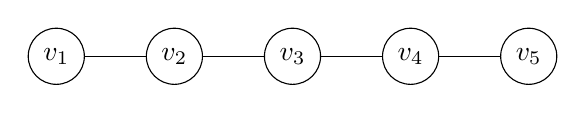
\begin{tikzpicture}[node distance={15mm}, main/.style = {draw, circle}]
		\node[main] (1) {$v_1$};
		\node[main] (2) [right of=1] {$v_2$};
		\node[main] (3) [right of=2] {$v_3$};
		\node[main] (4) [right of=3] {$v_4$};
		\node[main] (5) [right of=4] {$v_5$};
		\draw (1) -- (2);
		\draw (2) -- (3);
		\draw (3) -- (4);
		\draw (4) -- (5);
	\end{tikzpicture}
	\centering
	\caption{Graph $\mathfrak{G}_1$, consisting of a line of length $4$.}
\end{figure}